\subsection{Transformation to BPEL}
\label{sec:trafo_bpel}

The transformation to BPEL presented in this work covers nearly the entire mapping as given in the BPMN specification~\cite[Chapter 11]{omg2006business}, including event handlers, inclusive \textsc{or} and event-based \textsc{xor} Gateways, just to name a few.  Still there are some elements for which the mapping is not given very clearly, such as \textsc{timer} Start Events, independent Sub Processes or multi-instance parallel loops.  While these elements will be transformed as described in the specification, the resulting BPEL processes will require some amount of manual refinement.  Besides the BPEL process files a WSDL definitions file is created, holding the message types derived from the process properties and the input and output messages and interfaces (port types) for the several Web services being orchestrated by the process.  Still, the WSDL's binding and service blocks and necessary schema types, if any, can not be generated automatically yet, due to insufficient information in the source model.  We are currently investigating ways of extending the BPMN metamodel in order to include more information in the model and at the same time making it more independent of the BPEL language.

In the validation used for the transformation to BPEL, all identifiers are tested to contain only characters that are legal with respect to BPEL.  Additionally all expressions used e.g.\ in Assignments and loop conditions are scanned for occurrences of Property identifiers.  So if a Process \texttt{Proc} has a Property \texttt{foo} and there is an Assignment with an expression like \texttt{"foo+1"}, the expression will be changed to \texttt{"bpws:getVariableData('Proc\_ProcessData','foo')+1"}.  Thus the user does not have to care about the way Properties are represented with messages in BPEL but can use a Property's plain name in expressions.


\subsection{Example}
\label{sec:trafo_example}

The following example will show one of the scenarios being used in a smart home environment in the SerCHo project.  The resulting BPEL processes were validated and tested with the \emph{ActiveBPEL} designer and process engine.\footnote{\url{http://www.activebpel.org}}

The BPMN diagram in Figure~\ref{fig:example} is showing a ``Light Alarm'' process, that is used to open the blinds in the user's room to wake her up in a more pleasant way than the usual alarm clocks do.  For that purpose, firstly information on the current weather is retrieved using an external Web service.  Thereafter, based on the weather data, either the sunblinds are opened, or the ceiling light is turned on, or both.  In case the user does not get up, which is checked using an RFID based localisation solution, the stereo is turned on, playing her favourite song or alternatively an unpleasant alarm sound.

\begin{figure}%[htbp]
	\centering
	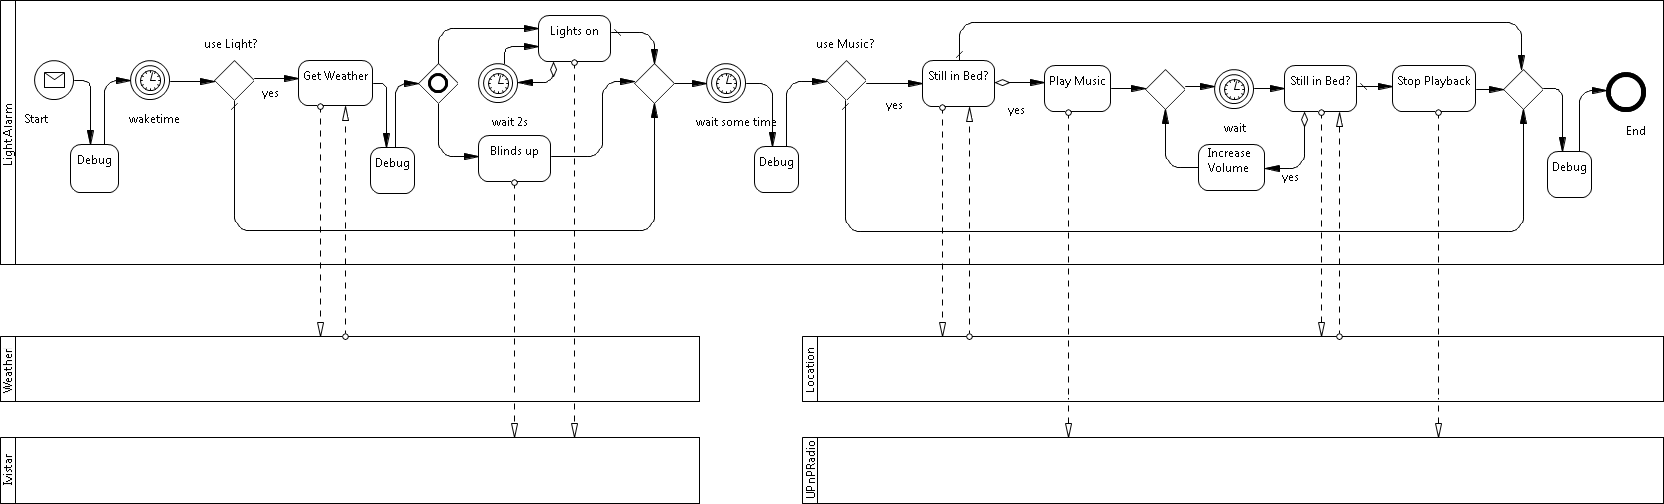
\includegraphics[width=\textwidth]{img/demo_lichtwecker_kompakt.png}
	\caption{``Light Alarm'' Example Process}
	\label{fig:example}
\end{figure}

For each of the above devices --- blinds, lights, localisation, and stereo --- Web service interfaces were written, so they can be integrated in a BPEL process.  While the WSDL file that is used by the process, holding the definitions for the various orchestrated services, has to be extended with the service bindings, the BPEL code resulting from this example is readily executable.


\subsection{Transformation to JIAC}
\label{sec:trafo_jiac}

Concerning our goal of transforming BPMN diagrams to multi-agent systems (MAS) the work is still at an early stage.  First, a \emph{normal form} for BPMN diagrams has been investigated, to facilitate the mapping~\cite{endert2007towards}.  Later, the first steps of the actual mapping have been developed, basically mapping Pools to agents, Processes and Flow Objects to the agents' plans and the control flow, and Message Flow to the exchange of messages between the agents~\cite{endert2007mapping}.

A first prototype targeting the agent framework JIAC IV~\cite{sesseler2002modularearchitektur} has already been implemented.  As the theoretical part of the mapping is not yet fully matured, there is still some work to do.  However, with the given transformation framework every addition to the mapping can quickly be adopted.
